\documentclass[11pt, oneside]{article} 
\usepackage{geometry}
\geometry{letterpaper} 
\usepackage{graphicx}
	
\usepackage{amssymb}
\usepackage{amsmath}
\usepackage{parskip}
\usepackage{color}
\usepackage{hyperref}

\graphicspath{{/Users/telliott/Github/calculus_book/png/}}
% \begin{center} 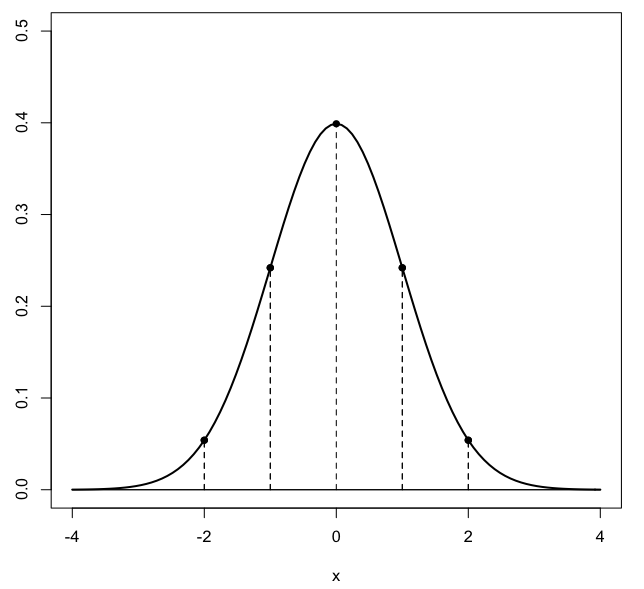
\includegraphics [scale=0.4] {gauss3.png} \end{center}

\title{Basic geometry and congruence of triangles}
\date{}

\begin{document}
\maketitle
\Large

\subsection*{Congruence and similarity}

$\circ$  Two triangles are \emph{congruent} if and only if they have the same three side lengths.  This is often abbreviated SSS (side-side-side).  

As we'll see, some other equalities are equivalent to (they imply) congruence and SSS equality.

By this definition, a triangle and its mirror image are congruent.  The three triangles shown below are all congruent, even though the first is flipped (it is the mirror image of the other two).

\begin{center} 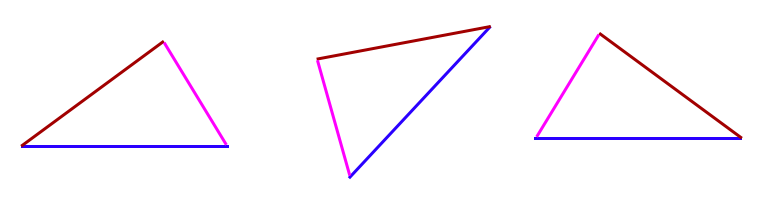
\includegraphics [scale=0.4] {congruent.png} \end{center}

Having the same three sides means that the shape is the same, and all three angles are the same --- the shapes are superimposable, with the proviso that we allow the shape to be flipped over.

In the next figure the two smaller triangles obtained by dividing in half an equilateral triangle (all sides equal), are congruent.  We will prove this later.

\begin{center} 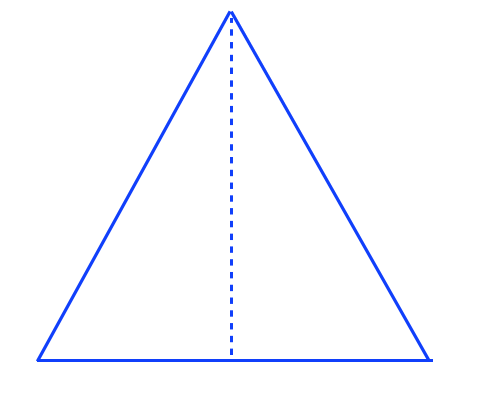
\includegraphics [scale=0.3] {congruent2.png} \end{center}

Some triangles are \emph{similar} but not congruent.

Similarity means that the three angles are the same but the triangles are of different overall sizes.  We might say that they are the same but \emph{scaled} differently.  

We can call this AAA (angle-angle-angle).  For similar triangles, the three corresponding pairs of sides are in the same proportions, but re-scaled by a constant of proportion.

$\circ$  Two triangles are similar if they have the same three angles. 

Because of the angle sum theorem, if any two angles of a pair of triangles are known to be equal, then the third one must be equal as well.

$\circ$  Two triangles are similar if they have two angles known to be equal. 

Similar triangles have their sides in the same proportions.

\begin{center} 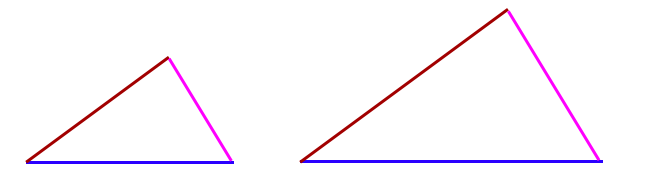
\includegraphics [scale=0.4] {similar.png} \end{center}

Given any triangle, draw a line parallel to one side, which also joins the other two sides.  The new triangle with that side as its base is similar to the given triangle.  Similarity means that all the angles are equal.  This is easily proved using the theorem on alternate interior angles.

\begin{center} 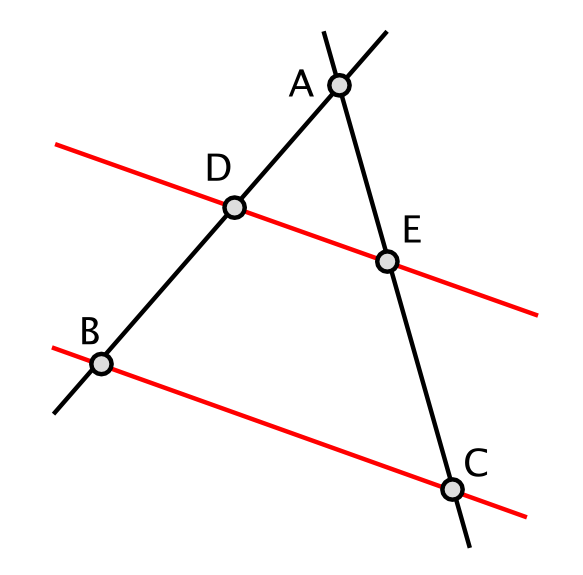
\includegraphics [scale=0.25] {Thales_theorem_1.png} \end{center}
%\begin{center} 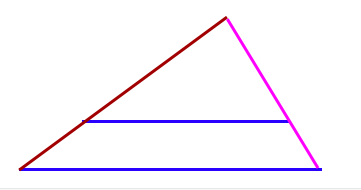
\includegraphics [scale=0.4] {parallel_line.png} \end{center}

In this example, these ratios are all equal
\[ \frac{AD}{AB} = \frac{AE}{AC} = \frac{DE}{BC}  \]
\[ \frac{AD}{DB} = \frac{AE}{EC} = \frac{DE}{BC - DE}  \]

In addition to SSS (side-side-side), there are three other conditions that lead to congruence of two triangles when they are satisfied, namely

$\circ$  SAS (side-angle-side)

$\circ$  ASA (angle-side-angle)

$\circ$  AAS (angle-angle-side)

\subsection*{constructions}

The way I think about these conditions is to imagine trying to construct a triangle from the given information, and ask whether it is uniquely determined.  Suppose we know ASA.  The situation is thus:

\begin{center} 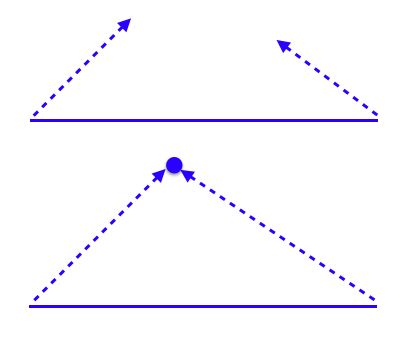
\includegraphics [scale=0.4] {ASA.png} \end{center}
 
Plot the known side using the known angles, start two other sides from the ends of that side.  They must cross at a unique point.  

But... actually, if we start the two lines pointing below the horizontal, there is another solution, the mirror image.  This triangle is also congruent to the one above.
 
\begin{center} 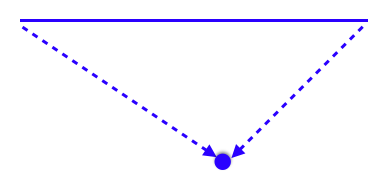
\includegraphics [scale=0.4] {ASA2.png} \end{center}

If we know two angles we also know the third, because they must add to 180 degrees.  For this reason, ASA and AAS imply that we have exactly the same information, because we know all three angles and (this part is important) we also know \emph{which} two angles flank the known side.

Alternatively, it is enough to know which angle faces a the known side.

\subsection*{one that doesn't work}

There is one set of three that doesn't work, that is ASS (angle-side-side).

\begin{center} 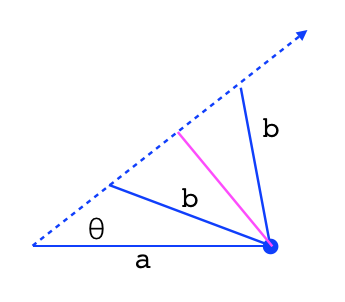
\includegraphics [scale=0.5] {angle_side_side.png} \end{center}

Here we know sides $a$ and $b$ and the angle $\theta$ adjacent to $a$ and facing opposite side $b$.  Imagine $b$ swinging on a hinge at the blue dot.  Since $b < a$, there are two points where $b$ can intersect with the side projecting from angle $\theta$.  There is no unique solution, so the triangle is not determined.

If it had been the case that $b > a$, or alternatively that $b$ formed a right angle with the third side, then the triangle \emph{would} be determined.

I think Tony Randall said it best

\url{https://www.youtube.com/watch?v=KEP1acj29-Y}

\subsection*{right triangles}
 
For two right-triangles, if the hypotenuses are equal and also one set of legs equal, the two triangles are congruent.

\begin{center} 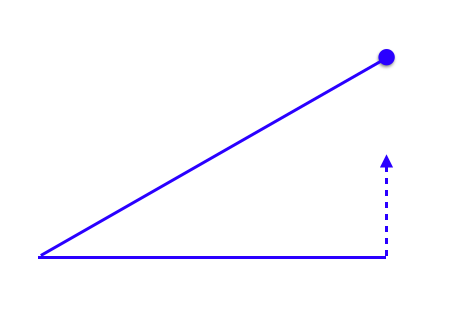
\includegraphics [scale=0.4] {hyp_side_congruent.png} \end{center}

In the figure, imagine the hypotenuse swinging on the hinge of its vertex with the horizontal base.  There is only one angle where it will terminate on the vertical side with the correct length.  This determines the angle between the known sides, or alternatively, the length of the third side.
 
\subsection*{another theorem from Thales}

$\circ$  The base angles of an isosceles triangle are equal.  Also, if the two base angles are equal, the triangle is isosceles.

\begin{center} 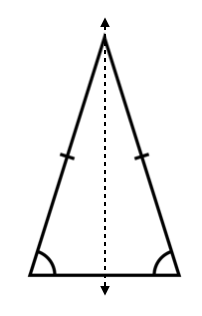
\includegraphics [scale=0.6] {isosceles.png} \end{center}

My favorite proof of this theorem is from symmetry (above).  Draw a line from the vertex between the two equal sides to the midpoint of the base opposite.  If you turn the triangle over along this axis, we obtain the same triangle back again.  

Alternatively, just say SSS or use the previous theorem on right triangles.

We prove this more carefully in the next chapter.

The theorem says that the base angles are equal $\iff$ the two sides sides (not the base) are equal.  The symbol $\iff$ means \emph{if and only if}, so $A \iff B$ means that both $A \rightarrow B$ and $B \rightarrow A$.

Above we said that in this figure the two smaller triangles obtained by dividing an equilateral triangle in half, are congruent.  The dotted line is called an \emph{altitude} of the triangle.
\begin{center} 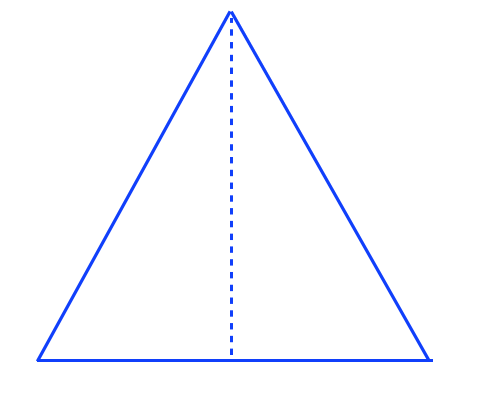
\includegraphics [scale=0.3] {congruent2.png} \end{center}

Because the left and right sides of the original triangle are equal, the base angles are equal, by the property of isosceles triangles which we just proved.  The angles where the altitude meets the base are both right angles, by symmetry and by the definition of the altitude.  Therefore we have AAS.

So, the two angles at the top where the altitude meets the sides are also equal (as the third angle when the other two angles are known).

\begin{center} 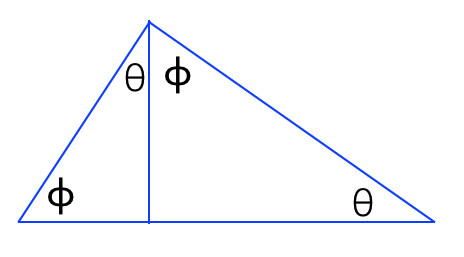
\includegraphics [scale=0.5] {right_triangle2.png} \end{center}
In any right triangle, if an altitude is dropped to the long side (called the \emph{hypotenuse}), then the two smaller triangles that are formed are similar to the original one.

The reason is that in any right triangle the two angles that are not the right angle add up to 90 degrees, so the whole will be 180 degrees.  These are called \emph{complementary} angles.

Each smaller triangle contains an angle also found in the large one.  Therefore the opposing, complementary angles are equal.

\subsection*{pyramid height}
As we said, Thales was from Miletus and he lived around 600 BC.  Thales is believed to have traveled extensively and was likely of Phoenician heritage.  As you probably know, the Phoenicians were famous sailors who founded many settlements around the Mediterranean.  

They competed with the mainland Greeks and later with the Romans for colonies, and their major city, Carthage, was destroyed much later by the Romans in the third Punic War.  

During his travels, Thales went to Egypt, home to the great pyramids at Giza, which were already ancient then.  They had been built just around around 2560 BC (dated by reference to Egyptian kings) and were already 2000 years old at that time!

The story is that Thales asked the Egyptian priests about the height of the Great Pyramid of Cheops, and they would not tell him.  So he set about measuring it himself.  The current height is 480 feet.  He used similar triangles.

\begin{center} 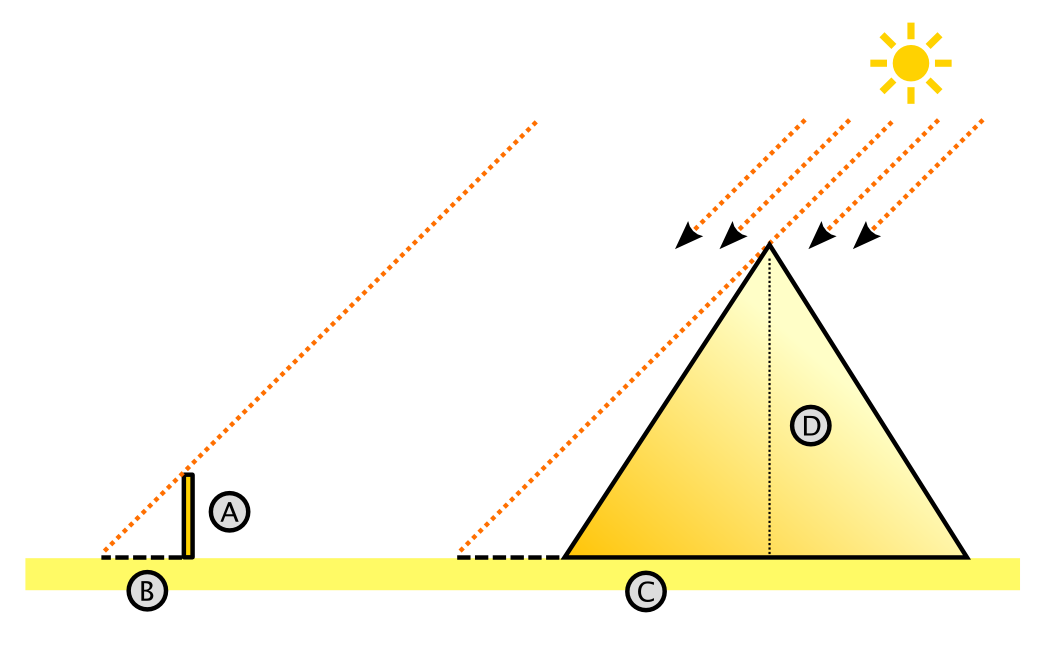
\includegraphics [scale=0.25] {Thales_theorem_6.png} \end{center}

\end{document}